\autsection{Use Case Diagrams}{Nelián Colón}
\label{sec:useCase}
\subsection*{Student}
\begin{figure}[H]
	\centering
	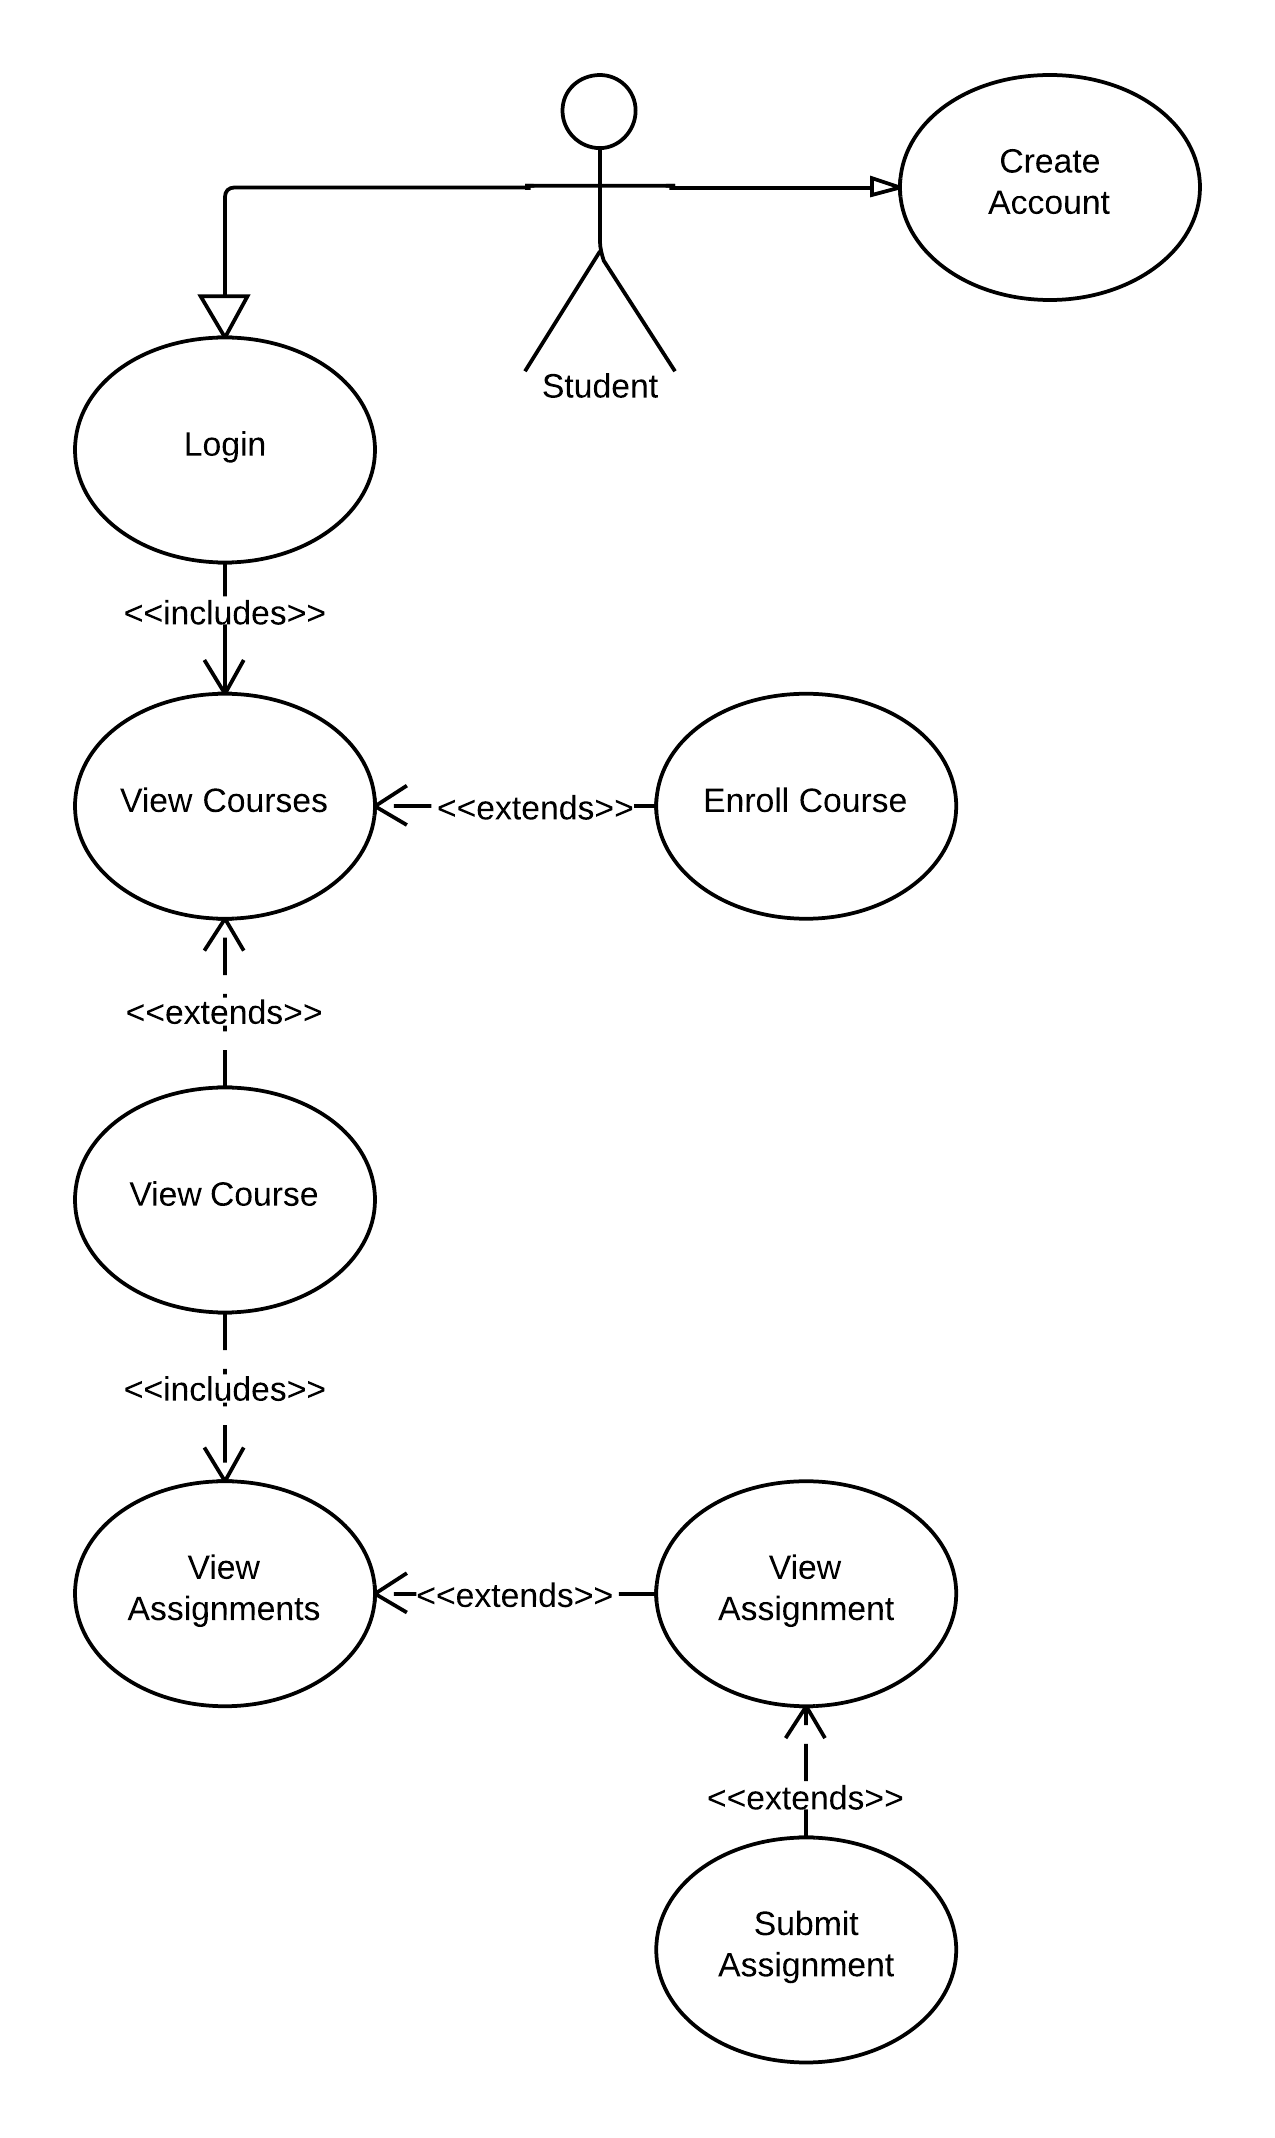
\includegraphics[scale=0.2]{img/useCaseStudent}
	\caption{Use Case Diagram - Student}
\end{figure}

\subsection*{Professor}
\begin{figure}[H]
	\centering
	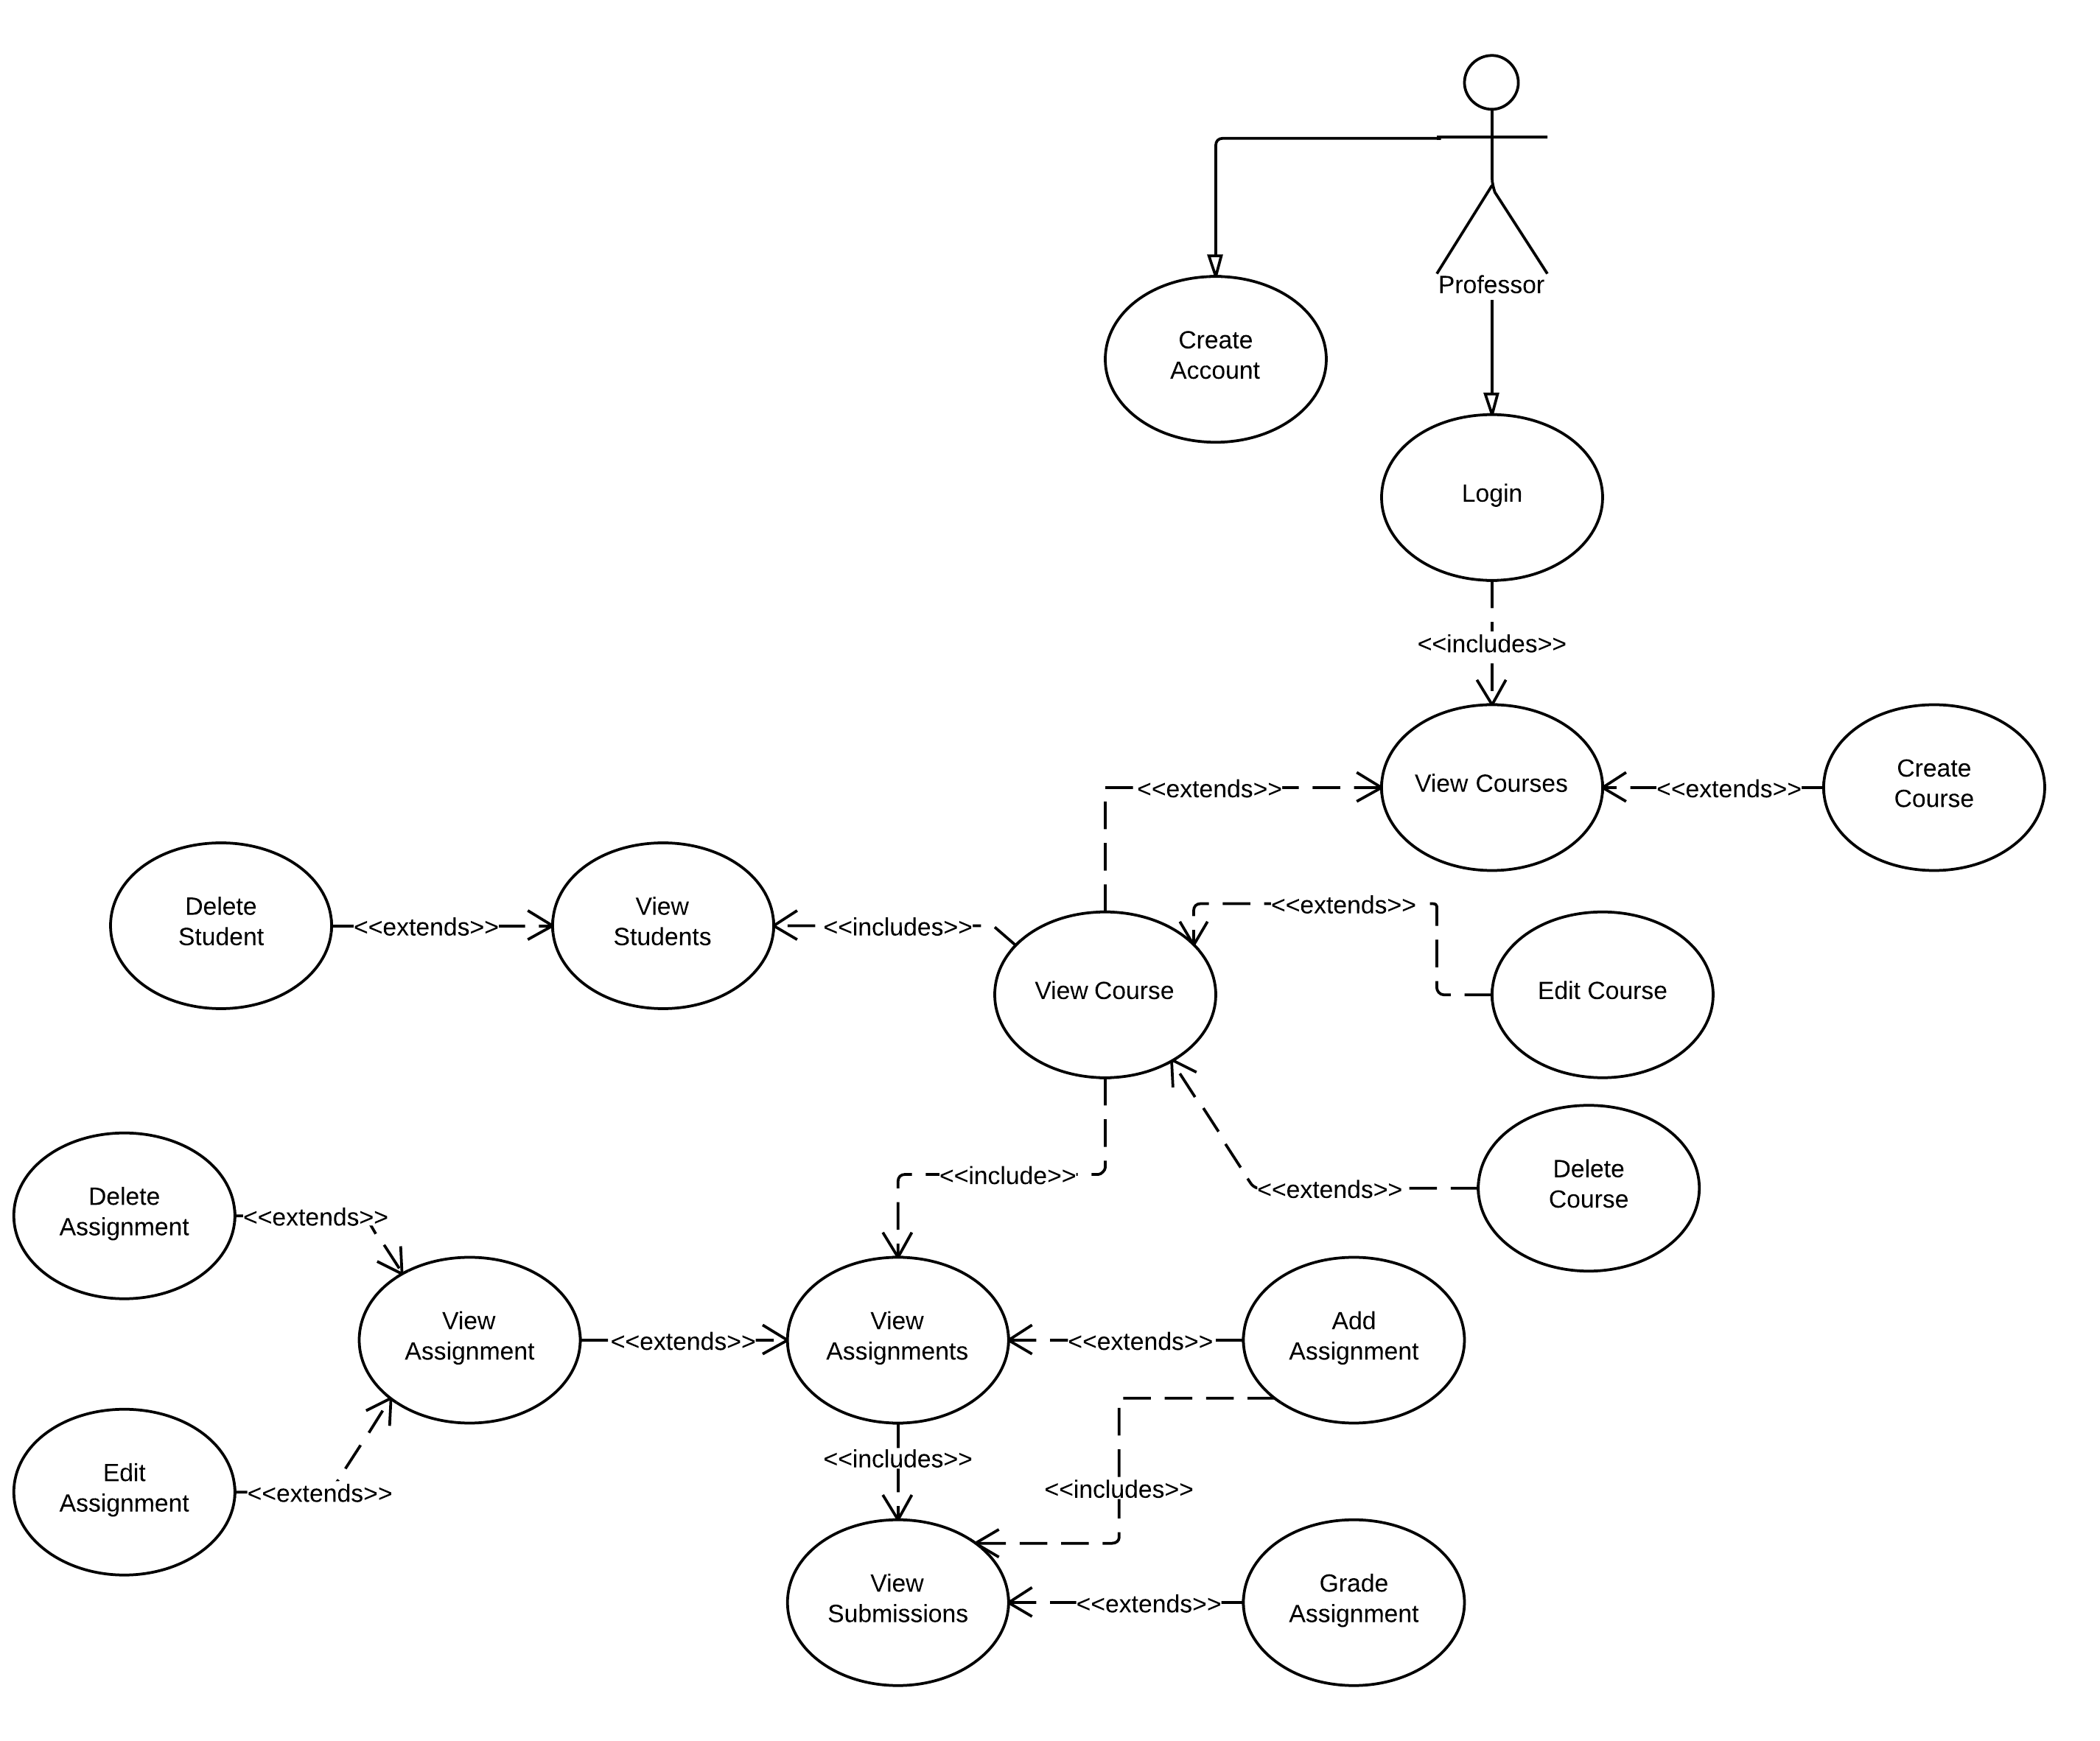
\includegraphics[width=\textwidth]{img/useCaseProf}
	\caption{Use Case Diagram - Professor}
\end{figure}

\subsection*{School Administrator}

\begin{figure}[H]
	\centering
	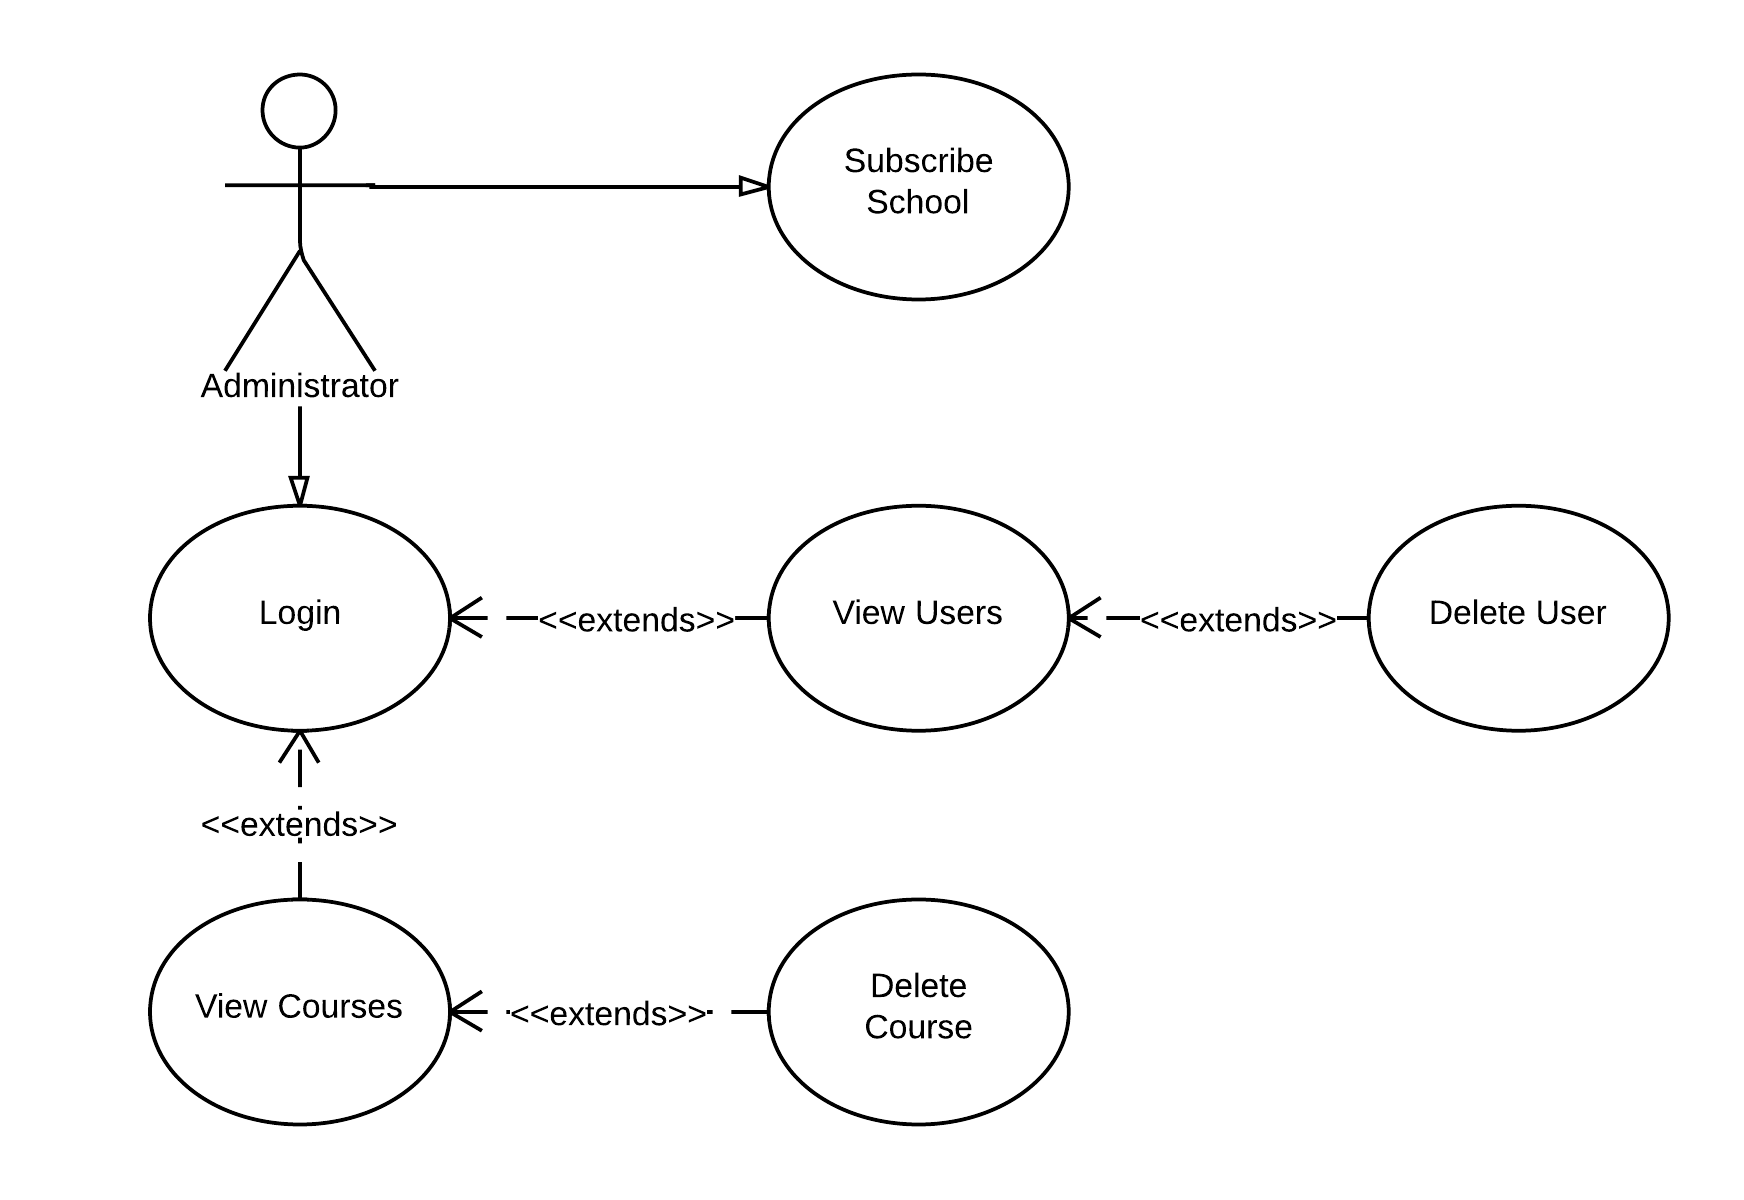
\includegraphics[width=\textwidth]{img/useCaseAdmin}
	\caption{Use Case Diagram - Administrator}
\end{figure}
\clearpage
\autsection{Use Case Descriptions}{Nelián Colón}
\label{sec:useCases}
\subsection*{Subscribe School}
Actors: School Administrator, System Administrator

Entry Condition: Administrator is in login page

Flow of events:

Basic Flow:

\begin{itemize}
\item School administrator selects the subscribe school option
\begin{itemize}
\item System sends email to system administrator
\end{itemize}
\item System administrator checks the solicitude
\begin{itemize}
\item If request is accepted, system sends email to administrator with 
login information. A rejection email is sent otherwise.
\end{itemize}
\end{itemize}
Exit condition: System is in login page

\subsection*{Approve Professor}
Actors: School Administrator

Entry Condition: Administrator is in home page

Flow of events:

Basic Flow:

\begin{itemize}
\item Administrator selects the view pending professor approvals options
\begin{itemize}
\item System shows a list of pending approvals
\end{itemize}
\item Administrator approves or disapproves a professor
\begin{itemize}
\item System gives professor access to professor and returns to 
pending approvals page
\end{itemize}
\end{itemize}
Exit condition: System is in pending approvals page



\textbf{Create Account}

Actors: Professor and Student

Entry Condition: Professor or student is in the login page.

Flow of events:

Basic Flow:

\begin{itemize}
\item User selects the Sign up option.
\begin{itemize}
\item System shows the signup page
\end{itemize}
\item User fills the information and creates an account if their school 
is available (with their @edu email).
\begin{itemize}
\item After creating an account, the user will be taken to the home 
page.
\item For both student and professor the will send confirmation email 
since no imposter students posing as professors are wanted.
\end{itemize}
\end{itemize}
Exit condition: The user is taken directly to his main account page.

Exceptions: The user already exists, password is too weak, invalid 
email, invalid password, school is not subscribed.

Special Requirements: The user must not already exist. If the user is 
not an administrator, then the school must not already be subscribed.

Notes/Issues: Make sure that a good subscribing model is used to prevent 
corruption (things like students creating admin / professors accounts, 
etc.)

\subsection*{Login}
Actors: Administrators, Students and Professors.

Entry point: The user is logged off and is in the homepage.

Basic Flow:

\begin{itemize}
\item User selects the login option
\begin{itemize}
\item System shows the login page
\end{itemize}
\item The user writes his email and password.
\begin{itemize}
\item If the login was successful, he is taken to his main account page. 

\end{itemize}
\end{itemize}
Exit Condition: The user is taken to his main account page.

Exceptions: Invalid Username or Password: an error message is 
shown.

Special Requirements: User must be logged off to see the login 
option

\subsection*{View Courses}
Actors: Students and Professors

Entry Condition: User is logged in

Flow of events:

Basic Flow:

\begin{itemize}
\item User goes to home page
\begin{itemize}
\item System displays a list of active courses
\end{itemize}
\end{itemize}
Exit condition: System is in home page

\subsection*{View Course}
Actors: Student, Professor

Entry Condition: User is logged in and is currently in the home 
page

Flow of events:

Basic Flow:

\begin{itemize}
\item User selects the course that wants to see
\begin{itemize}
\item System displays course information page
\end{itemize}
\end{itemize}
Exit condition: System is in course information page

\subsection*{Add Course}
Actors: Professors

Entry Condition: Professor is in home page

Flow of events:

Basic Flow:

\begin{itemize}
\item Professor selects the add course option
\begin{itemize}
\item System displays the add course page
\end{itemize}
\item Professor submits the information and confirms
\begin{itemize}
\item System returns to home page
\end{itemize}
\end{itemize}
Exit condition: System is in home page

\subsection*{Edit Course}\label{section:h.vwpc5v6194kl}
Actors: Professor

Entry Condition: Professor is logged in and is in view course 
page

Flow of events:

Basic Flow:

\begin{itemize}
\item Professor selects the edit course option
\begin{itemize}
\item System displays edit course page
\end{itemize}
\item Professor makes changes, submits the information and confirms the 
changes
\begin{itemize}
\item System updates the course and returns to view course page
\end{itemize}
\end{itemize}
Exit condition: System is in view course screen

\subsection*{Delete Course}\label{section:h.u6yi7m9pwom7}
Actors: Professor

Entry Condition: Professor is logged in and is in home page

Flow of events:

Basic Flow:

\begin{itemize}
\item Professor selects the delete course option
\begin{itemize}
\item System pop ups a confirmation message
\end{itemize}
\item Professor confirms the deletion
\begin{itemize}
\item System deletes the course from the home page
\end{itemize}
\end{itemize}

Exit condition: System is in home page



\subsection*{Enroll in course}\label{section:h.rjvrpx5d6ohf}
Actors: Students

Entry Condition: The Student or teaching assistant is in the main page. 

Flow of Events:

Basic Flow:

\begin{itemize}
\item The student selects the add course option
\begin{itemize}
\item The system displays the add course page
\end{itemize}
\item Student selects the desired course
\begin{itemize}
\item System asks for course password
privileges.
\end{itemize}
\item Student inputs password
\begin{itemize}
\item If the password is correct, the course is enrolled. If it is incorrect, an error message is displayed. The system returns to the previous page.
\end{itemize}
\end{itemize}
Exit Condition: The student successfully enrolled the course and is 
taken to the home page.

\subsection*{View Assignments}\label{section:h.7pxq6fih8yfa}
Actors: Student, Professor

Entry Condition: User is logged in and is in view course page

Flow of events: 

Basic Flow:

\begin{itemize}
\item User selects the view assignments option
\begin{itemize}
\item System displays a list of assignments with basic information
\end{itemize}
\end{itemize}

Exit condition: System is in view assignments screen

\subsection*{View assignment}\label{section:h.4ha1yl1avqpu}
Actors: Students, Professors

Entry Point: User is logged in and is on the view assignments page

Basic Flow:

\begin{itemize}
\item User clicks on the desired assignment
\begin{itemize}
\item System displays the assignment information
\end{itemize}
\item User closes the assignment when done
\begin{itemize}
\item System returns to view assignments
\end{itemize}
\end{itemize}

Exit Condition: System is in the view assignments screen

\subsection*{Submit Assignment}\label{section:h.tog3atpf2tbl}
Actors: Students

Entry Condition: Student is in the view assignment screen

Flow of events:

Basic Flow:

\begin{itemize}
\item Student selects the submit assignment screen
\begin{itemize}
\item System finds the necessary repository and displays a confirmation 
page
\end{itemize}
\item Student confirms the submission
\begin{itemize}
\item System submits the assignment for grading and returns to view 
assignment screen
\end{itemize}
\end{itemize}
Alternative Flow:

Exit condition: System is in view assignment screen

\subsection*{Add Assignment}\label{section:h.y1nuewn5cyxy}
Actors: Professor

Entry Point: The professor is logged in and is on the view 
assignments screen.

Basic Flow:

\begin{itemize}
\item Professor selects add assignment option
\begin{itemize}
\item System displays the add assignment form
\end{itemize}
\item Professor fills the information and adds test cases, then selects 
the submit option as a confirmation
\begin{itemize}
\item System adds assignment to course and returns to view assignments 
screen
\end{itemize}
\end{itemize}
Exit Condition: System is in the view assignments screen

\subsection*{Grade}\label{section:h.b0103s5vycbq}
Actors: Professors

Entry Condition: The professor is logged in and is on the view 
submissions page

Flow of events:

Basic Flow

\begin{itemize}
\item Professor selects a submission
\begin{itemize}
\item System shows professor the submission with a preliminary grade and 
quality check
\end{itemize}
\item Professor revises grade, adds comments to code and puts final 
grade
\begin{itemize}
\item System asks for confirmation of final grade
\end{itemize}
\item Professor confirms the grade
\begin{itemize}
\item System puts the grade in the student account and returns to view 
submissions page
\end{itemize}
\end{itemize}
Exit Condition: System is in the submission page

Special Requirements: The student must have submitted code for 
it to be graded.

Notes/Issues: None

\subsection*{Delete Assignment}\label{section:h.gw7q7yjp1gn9}
Actors: Professor

Entry Condition: Professor is logged in and is on the view 
assignments page

Flow of events:

Basic Flow:

\begin{itemize}
\item Professor selects the delete assignment option
\begin{itemize}
\item Systems asks for confirmation
\end{itemize}
\item Professor confirms deletion
\begin{itemize}
\item System deletes assignment and returns to view assignment page
\end{itemize}
\end{itemize}
Exit condition: System is in view assignment page

\subsection*{Edit Assignment}\label{section:h.bdm7ybz2uvl4}
Actors: Professor

Entry Condition: Professor is logged in and is on the view 
assignment page

Flow of events:

Basic Flow:

\begin{itemize}
\item Professor selects the edit assignment option
\begin{itemize}
\item System displays the edit assignment page
\end{itemize}
\item Professor makes changes, submits the information and confirms the 
changes
\begin{itemize}
\item System updates the assignment and returns to view assignment page
\end{itemize}
\end{itemize}
Exit condition: System is in the view assignment page

\subsection*{View Submissions}\label{section:h.sdxmdqspwi1p}
Actors: Professor

Entry Condition: Professor is logged in and is on the view 
assignment page

Flow of events:

Basic Flow:

\begin{itemize}
\item Professor selects the view submissions option
\begin{itemize}
\item System displays the submissions for the specific assignment
\end{itemize}
\end{itemize}
Exit condition: System is in the view submissions page

\subsection*{View Students}\label{section:h.ehmhdybzzy6b}
Actors: Professor

Entry Condition: Professor is logged in and is in view course 
page

Flow of events:

Basic Flow:

\begin{itemize}
\item Professor selects the view students option
\begin{itemize}
\item System displays a list of students with their information
\end{itemize}
\end{itemize}
Exit condition: System is in view students page